% !TeX root = exercise07.tex
\documentclass[a4paper,11pt]{article}
\usepackage{a4wide}
\usepackage{graphicx}
\usepackage[T1]{fontenc}
\usepackage[latin1]{inputenc}
%\usepackage[utf8]{inputenc}
\usepackage{ae}
\usepackage{url}
\usepackage{enumerate}
\usepackage{float}
\usepackage{amsmath}
\usepackage{subfigure}
\usepackage{color}
\usepackage{listings}
\usepackage[final]{pdfpages}
\usepackage{floatflt}
\usepackage{booktabs}
\usepackage{epstopdf}
\usepackage{graphicx, array, blindtext}
\usepackage{fancyhdr}
\usepackage{hyperref}
\usepackage{enumitem}
\usepackage{xcolor}
\usepackage{fancyvrb}

\font\helvSmallMediumFont=phvr at 4.0mm
\font\helvSmallBoldFont=phvb at 4.0mm
\font\helvMediumFont=phvr at 4.3mm
\font\helvBoldFont=phvb at 4.3mm
\font\ncsLargeFont=pncr at 5.0mm
\def\helvSmall{\helvSmallBoldFont\baselineskip=3mm}
\def\helvMedium{\helvMediumFont\baselineskip=6mm}
\def\ncsLarge{\ncsLargeFont\baselineskip=21mm}

\sloppy

\pagestyle{empty}

\definecolor{mygreen}{rgb}{0,0.6,0}
\definecolor{mygray}{rgb}{0.5,0.5,0.5}
\definecolor{mymauve}{rgb}{0.58,0,0.82}

\lstset{
  basicstyle=\color{white}\ttfamily,
  breaklines=true,
  backgroundcolor=\color{black},
  frame=none,
  columns=fullflexible
}

\setlist{noitemsep,topsep=5pt,parsep=0pt,partopsep=0pt}

\setlength{\parindent}{0px}

\begin{document}
\newcommand{\dozenten}{Prof.~Dr.~Steffen Herbold}
\newcommand{\vorlesung}{Principles of AI Engineering}
\newcommand{\docauthor}{Lukas Schulte}
\newcommand{\semester}{}
\newcommand{\blattnummer}{7}
\newcommand{\bistermin}{}
\addtolength{\topmargin}{-2cm}
\noindent

\begin{table}[ht]
    \centering
    \begin{tabular}{*{2}{m{0.48\textwidth}}}
        \helvBoldFont \vorlesung \helvMedium


        \vspace{1ex}
        \helvBoldFont Exercise \blattnummer


        \vspace{1ex}
        \dozenten


        \helvMedium\semester

         &
        
\includegraphics[width=0.45\textwidth]{common/aie_square.png}
    \end{tabular}
\end{table}
\vspace{-1.75cm}
\hrule width \columnwidth
\begin{flushright}
    \vspace{-0.25cm}
    \small Author: \docauthor
    \vspace{-0.75cm}
\end{flushright}


\section*{Project task}
% Client application

Create a client application that must consume your REST API. This may be a web application or a native application. The important requirement is, that it uses the REST API of your server application.

\vspace{5px}

You can find a sketch for the UI below. Modify it at your own discretion.

\vspace{5px}

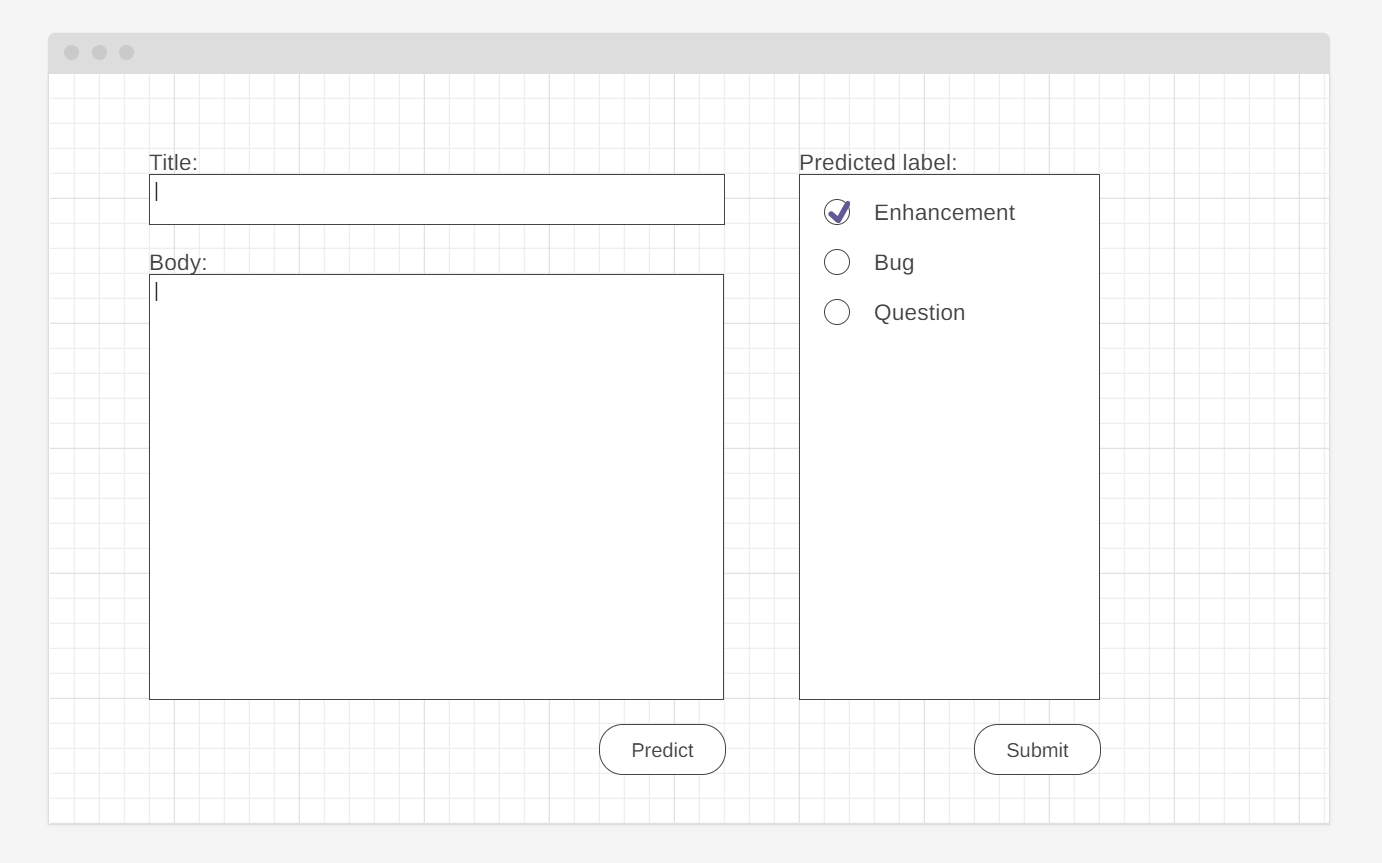
\includegraphics[width=\linewidth]{upPrinciplesAIEWireframe.png}

\section*{Questions}

\begin{enumerate}
      \item
            Describe how you would design the deployment architecture from the problem description. You can make assumptions, e.g., data/model size where appropriate.
            Include information on where the model is deployed, opportunities for telemetry, update times, latency.
      \item
            What would be the advantages and disadvantages of deploying the application with a microservice architecture?
\end{enumerate}

\end{document}
